\subsection{Experimental}

\begin{frame}{Hard spheres and colloids}
	\begin{textblock*}{0.6\textwidth}(10mm,92mm)
		\only<2>{\simplephasediagram{}}%
	\end{textblock*}
	The volume fraction $\phi$ is like an inverse temperature.
	\bigskip
	\def\svgwidth{\textwidth}\input{phase_diagram.pdf_tex}
	
	\bigskip
	Well approximated by sterically stabilised colloids\\
	\begin{footnotesize}\citep{pusey1986}\end{footnotesize}
\end{frame}

\begin{frame}{Our colloids}
	\begin{columns}
	\column{0.5\textwidth}
	\centering
	\rotatebox{90}{\qquad \small{SEM image}}\includegraphics[width=0.8\columnwidth]{SEM}\\
	\resizebox{\columnwidth}{!}{\begin{huge}% GNUPLOT: LaTeX picture with Postscript
\begingroup
  \makeatletter
  \providecommand\color[2][]{%
    \GenericError{(gnuplot) \space\space\space\@spaces}{%
      Package color not loaded in conjunction with
      terminal option `colourtext'%
    }{See the gnuplot documentation for explanation.%
    }{Either use 'blacktext' in gnuplot or load the package
      color.sty in LaTeX.}%
    \renewcommand\color[2][]{}%
  }%
  \providecommand\includegraphics[2][]{%
    \GenericError{(gnuplot) \space\space\space\@spaces}{%
      Package graphicx or graphics not loaded%
    }{See the gnuplot documentation for explanation.%
    }{The gnuplot epslatex terminal needs graphicx.sty or graphics.sty.}%
    \renewcommand\includegraphics[2][]{}%
  }%
  \providecommand\rotatebox[2]{#2}%
  \@ifundefined{ifGPcolor}{%
    \newif\ifGPcolor
    \GPcolortrue
  }{}%
  \@ifundefined{ifGPblacktext}{%
    \newif\ifGPblacktext
    \GPblacktexttrue
  }{}%
  % define a \g@addto@macro without @ in the name:
  \let\gplgaddtomacro\g@addto@macro
  % define empty templates for all commands taking text:
  \gdef\gplbacktext{}%
  \gdef\gplfronttext{}%
  \makeatother
  \ifGPblacktext
    % no textcolor at all
    \def\colorrgb#1{}%
    \def\colorgray#1{}%
  \else
    % gray or color?
    \ifGPcolor
      \def\colorrgb#1{\color[rgb]{#1}}%
      \def\colorgray#1{\color[gray]{#1}}%
      \expandafter\def\csname LTw\endcsname{\color{white}}%
      \expandafter\def\csname LTb\endcsname{\color{black}}%
      \expandafter\def\csname LTa\endcsname{\color{black}}%
      \expandafter\def\csname LT0\endcsname{\color[rgb]{1,0,0}}%
      \expandafter\def\csname LT1\endcsname{\color[rgb]{0,1,0}}%
      \expandafter\def\csname LT2\endcsname{\color[rgb]{0,0,1}}%
      \expandafter\def\csname LT3\endcsname{\color[rgb]{1,0,1}}%
      \expandafter\def\csname LT4\endcsname{\color[rgb]{0,1,1}}%
      \expandafter\def\csname LT5\endcsname{\color[rgb]{1,1,0}}%
      \expandafter\def\csname LT6\endcsname{\color[rgb]{0,0,0}}%
      \expandafter\def\csname LT7\endcsname{\color[rgb]{1,0.3,0}}%
      \expandafter\def\csname LT8\endcsname{\color[rgb]{0.5,0.5,0.5}}%
    \else
      % gray
      \def\colorrgb#1{\color{black}}%
      \def\colorgray#1{\color[gray]{#1}}%
      \expandafter\def\csname LTw\endcsname{\color{white}}%
      \expandafter\def\csname LTb\endcsname{\color{black}}%
      \expandafter\def\csname LTa\endcsname{\color{black}}%
      \expandafter\def\csname LT0\endcsname{\color{black}}%
      \expandafter\def\csname LT1\endcsname{\color{black}}%
      \expandafter\def\csname LT2\endcsname{\color{black}}%
      \expandafter\def\csname LT3\endcsname{\color{black}}%
      \expandafter\def\csname LT4\endcsname{\color{black}}%
      \expandafter\def\csname LT5\endcsname{\color{black}}%
      \expandafter\def\csname LT6\endcsname{\color{black}}%
      \expandafter\def\csname LT7\endcsname{\color{black}}%
      \expandafter\def\csname LT8\endcsname{\color{black}}%
    \fi
  \fi
  \setlength{\unitlength}{0.0500bp}%
  \begin{picture}(7200.00,5040.00)%
    \gplgaddtomacro\gplbacktext{%
      \csname LTb\endcsname%
      \put(1342,704){\makebox(0,0)[r]{\strut{}$0$}}%
      \put(1342,1286){\makebox(0,0)[r]{\strut{}$0.05$}}%
      \put(1342,1867){\makebox(0,0)[r]{\strut{}$0.10$}}%
      \put(1342,2449){\makebox(0,0)[r]{\strut{}$0.15$}}%
      \put(1342,3030){\makebox(0,0)[r]{\strut{}$0.20$}}%
      \put(1342,3612){\makebox(0,0)[r]{\strut{}$0.25$}}%
      \put(1342,4193){\makebox(0,0)[r]{\strut{}$0.30$}}%
      \put(1342,4775){\makebox(0,0)[r]{\strut{}$0.35$}}%
      \put(1474,484){\makebox(0,0){\strut{}$2$}}%
      \put(2148,484){\makebox(0,0){\strut{}$2.2$}}%
      \put(2823,484){\makebox(0,0){\strut{}$2.4$}}%
      \put(3497,484){\makebox(0,0){\strut{}$2.6$}}%
      \put(4172,484){\makebox(0,0){\strut{}$2.8$}}%
      \put(4846,484){\makebox(0,0){\strut{}$3$}}%
      \put(5520,484){\makebox(0,0){\strut{}$3.2$}}%
      \put(6195,484){\makebox(0,0){\strut{}$3.4$}}%
      \put(6869,484){\makebox(0,0){\strut{}$3.6$}}%
      \put(308,2739){\rotatebox{-270}{\makebox(0,0){\strut{}Probability}}}%
      \put(4171,154){\makebox(0,0){\strut{}$\sigma$ (in \micro\meter)}}%
    }%
    \gplgaddtomacro\gplfronttext{%
    }%
    \gplbacktext
    \put(0,0){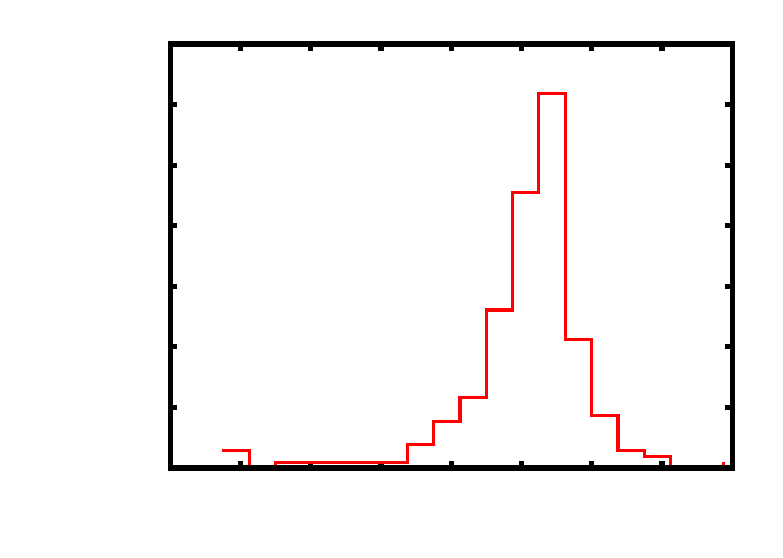
\includegraphics{diameter_histogram}}%
    \gplfronttext
  \end{picture}%
\endgroup
\end{huge}}
	\column{0.5\textwidth}
	\begin{itemize}
		\item PMMA particles 
		\begin{itemize}
			\item $\sigma \simeq \unit{3.3}{\micro\metre}$
			\item $\Delta \simeq 6\%$ not Gaussian
		\end{itemize}
		\item Hard spheres
		\begin{itemize}
			\item Sterically stabilized
			\item Salt to screen charges\\ (Debye length $<\unit{100}{\nano}{\metre}$)
		\end{itemize}
		\item Solvent
		\begin{itemize}
			\item Cis-decalin
			\item Cyclohexylbromide
		\end{itemize}
		\item Matching
		\begin{itemize}
			\item Optical index
			\item Density (with $T$ control)
		\end{itemize}
	\end{itemize}
	\end{columns}
\end{frame}

\begin{frame}{Confocal microscopy}
	\begin{columns}
	\column{0.4\textwidth}
	\def\svgwidth{\columnwidth}\input{confocalprinciple_vertical.pdf_tex}
	\column{0.6\textwidth}
	\centering
	$XY$ slice\quad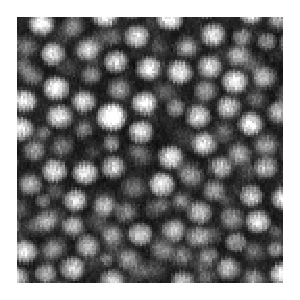
\includegraphics[width=0.5\columnwidth]{sliceXY}  
	
	\bigskip
	$XZ$ slice\quad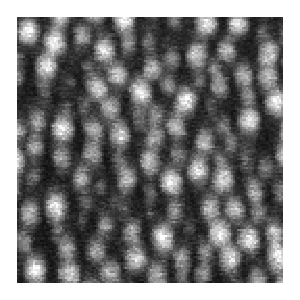
\includegraphics[width=0.5\columnwidth]{sliceXZ}
	\end{columns}
\end{frame}

\subsection{Tracking}
\begin{frame}{Particle tracking}
	\begin{columns}[T]
	\column{0.3\textwidth}
	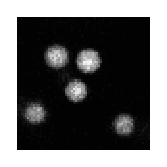
\includegraphics[width=\textwidth]{dillute_raw}
	
	\bigskip
	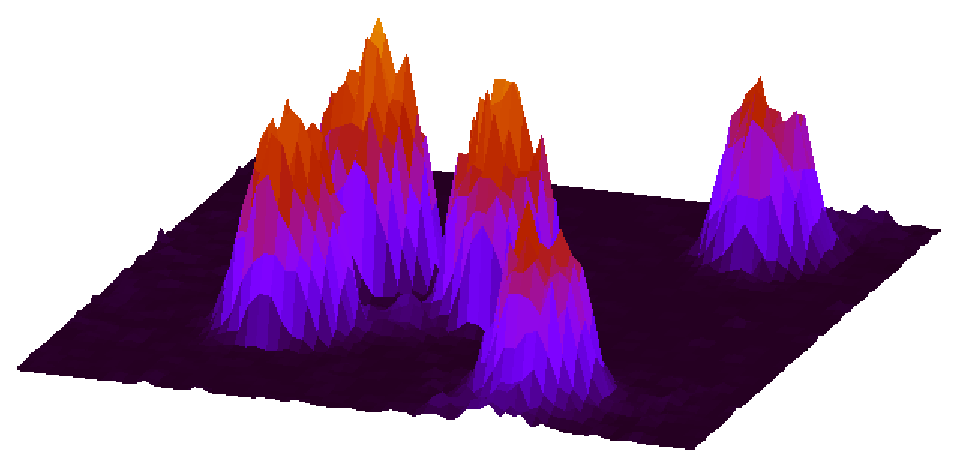
\includegraphics[width=\textwidth]{dillute_raw_gp_raster}
	\column{0.3\textwidth}
	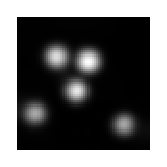
\includegraphics[width=\textwidth]{dillute_filtered}
	
	\bigskip
	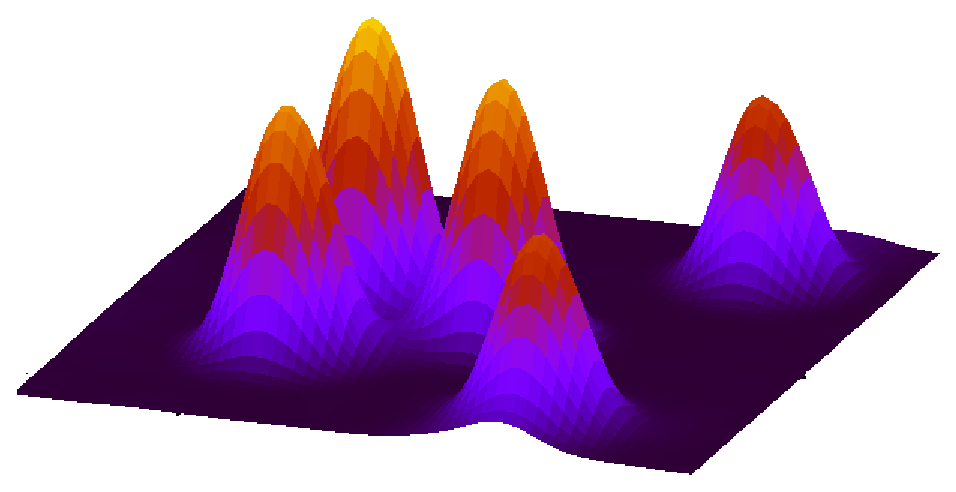
\includegraphics[width=\textwidth]{dillute_filtered_gp_raster}
	\column{0.3\textwidth}
	
\includegraphics[width=\textwidth]{dillute_centers}
	
	\bigskip
	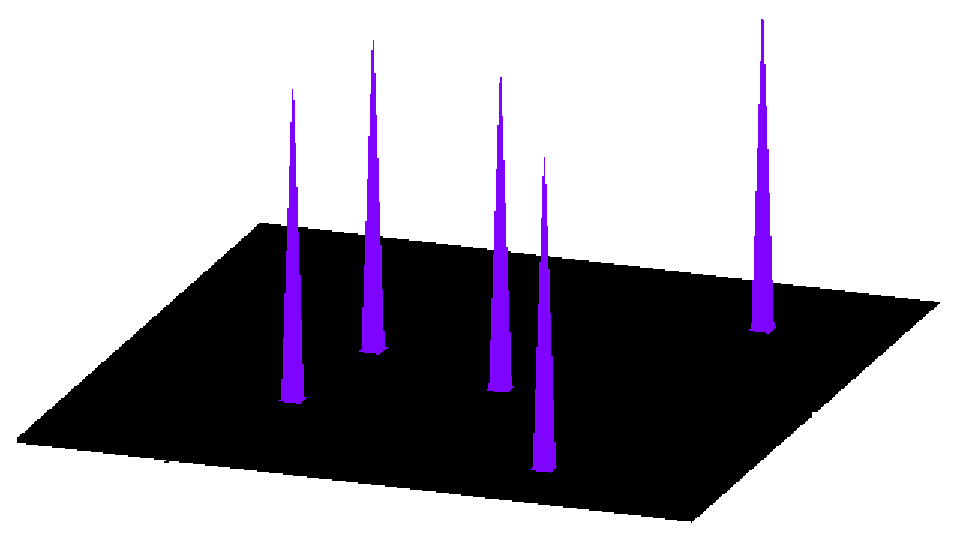
\includegraphics[width=\textwidth]{dillute_centers_gp_raster}
	\end{columns}
	
	\bigskip
	\[ (\unit{512}{pixels})^3 \xrightarrow{\unit{4}{\second}} \unit{5\times 10^4}{particles} \]
\end{frame}

\begin{frame}{Tracking accuracy}
	\begin{columns}
	\column{0.7\textwidth}
	\only<1|handout:0>{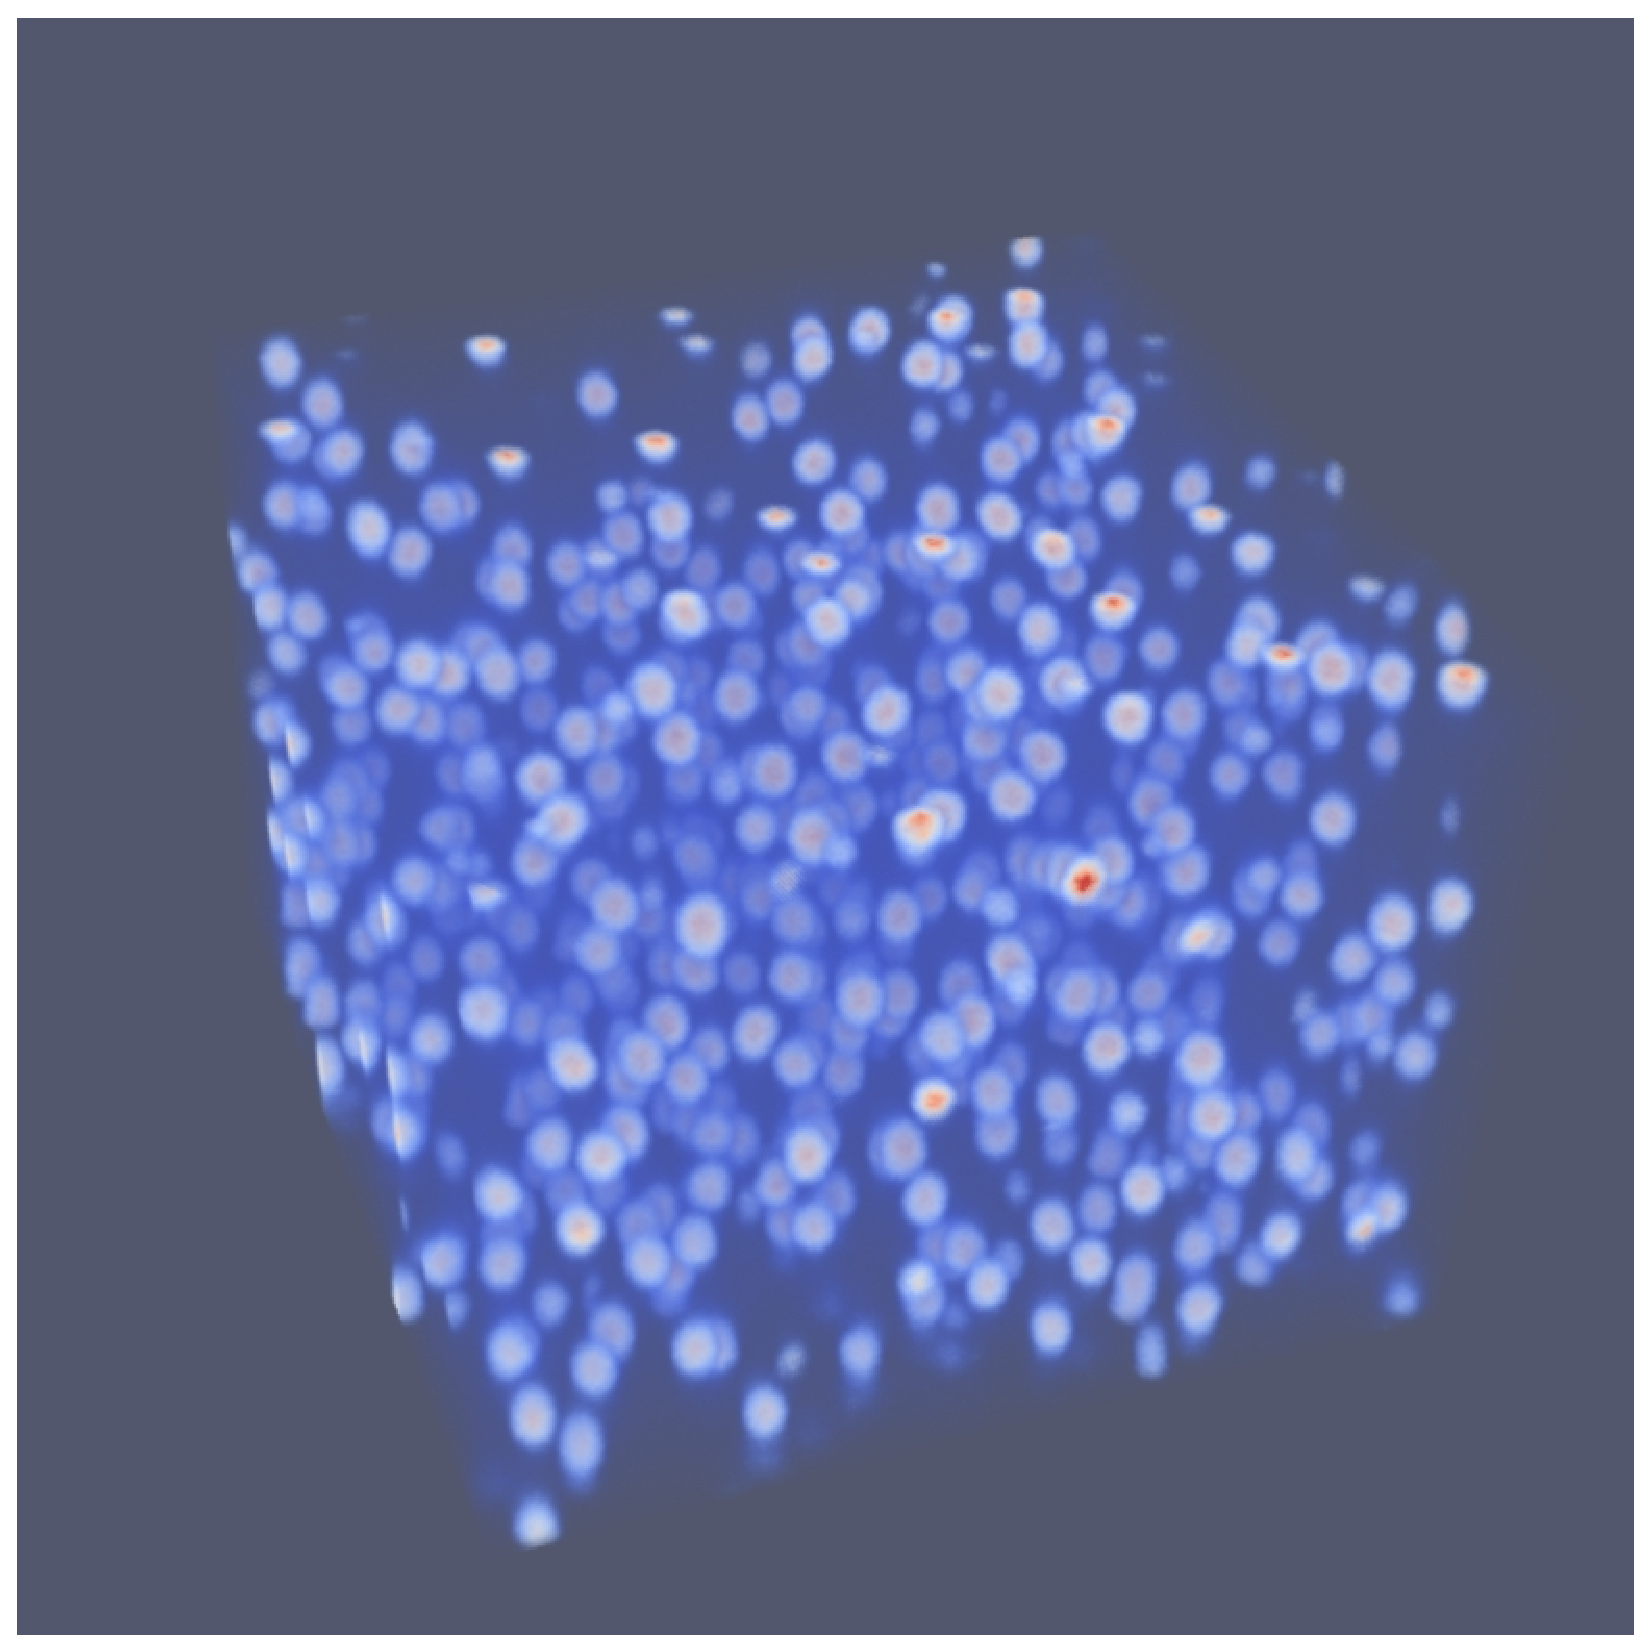
\includegraphics[width=\columnwidth]{compare_image_tracked3D_0}}%
	\only<2|handout:0>{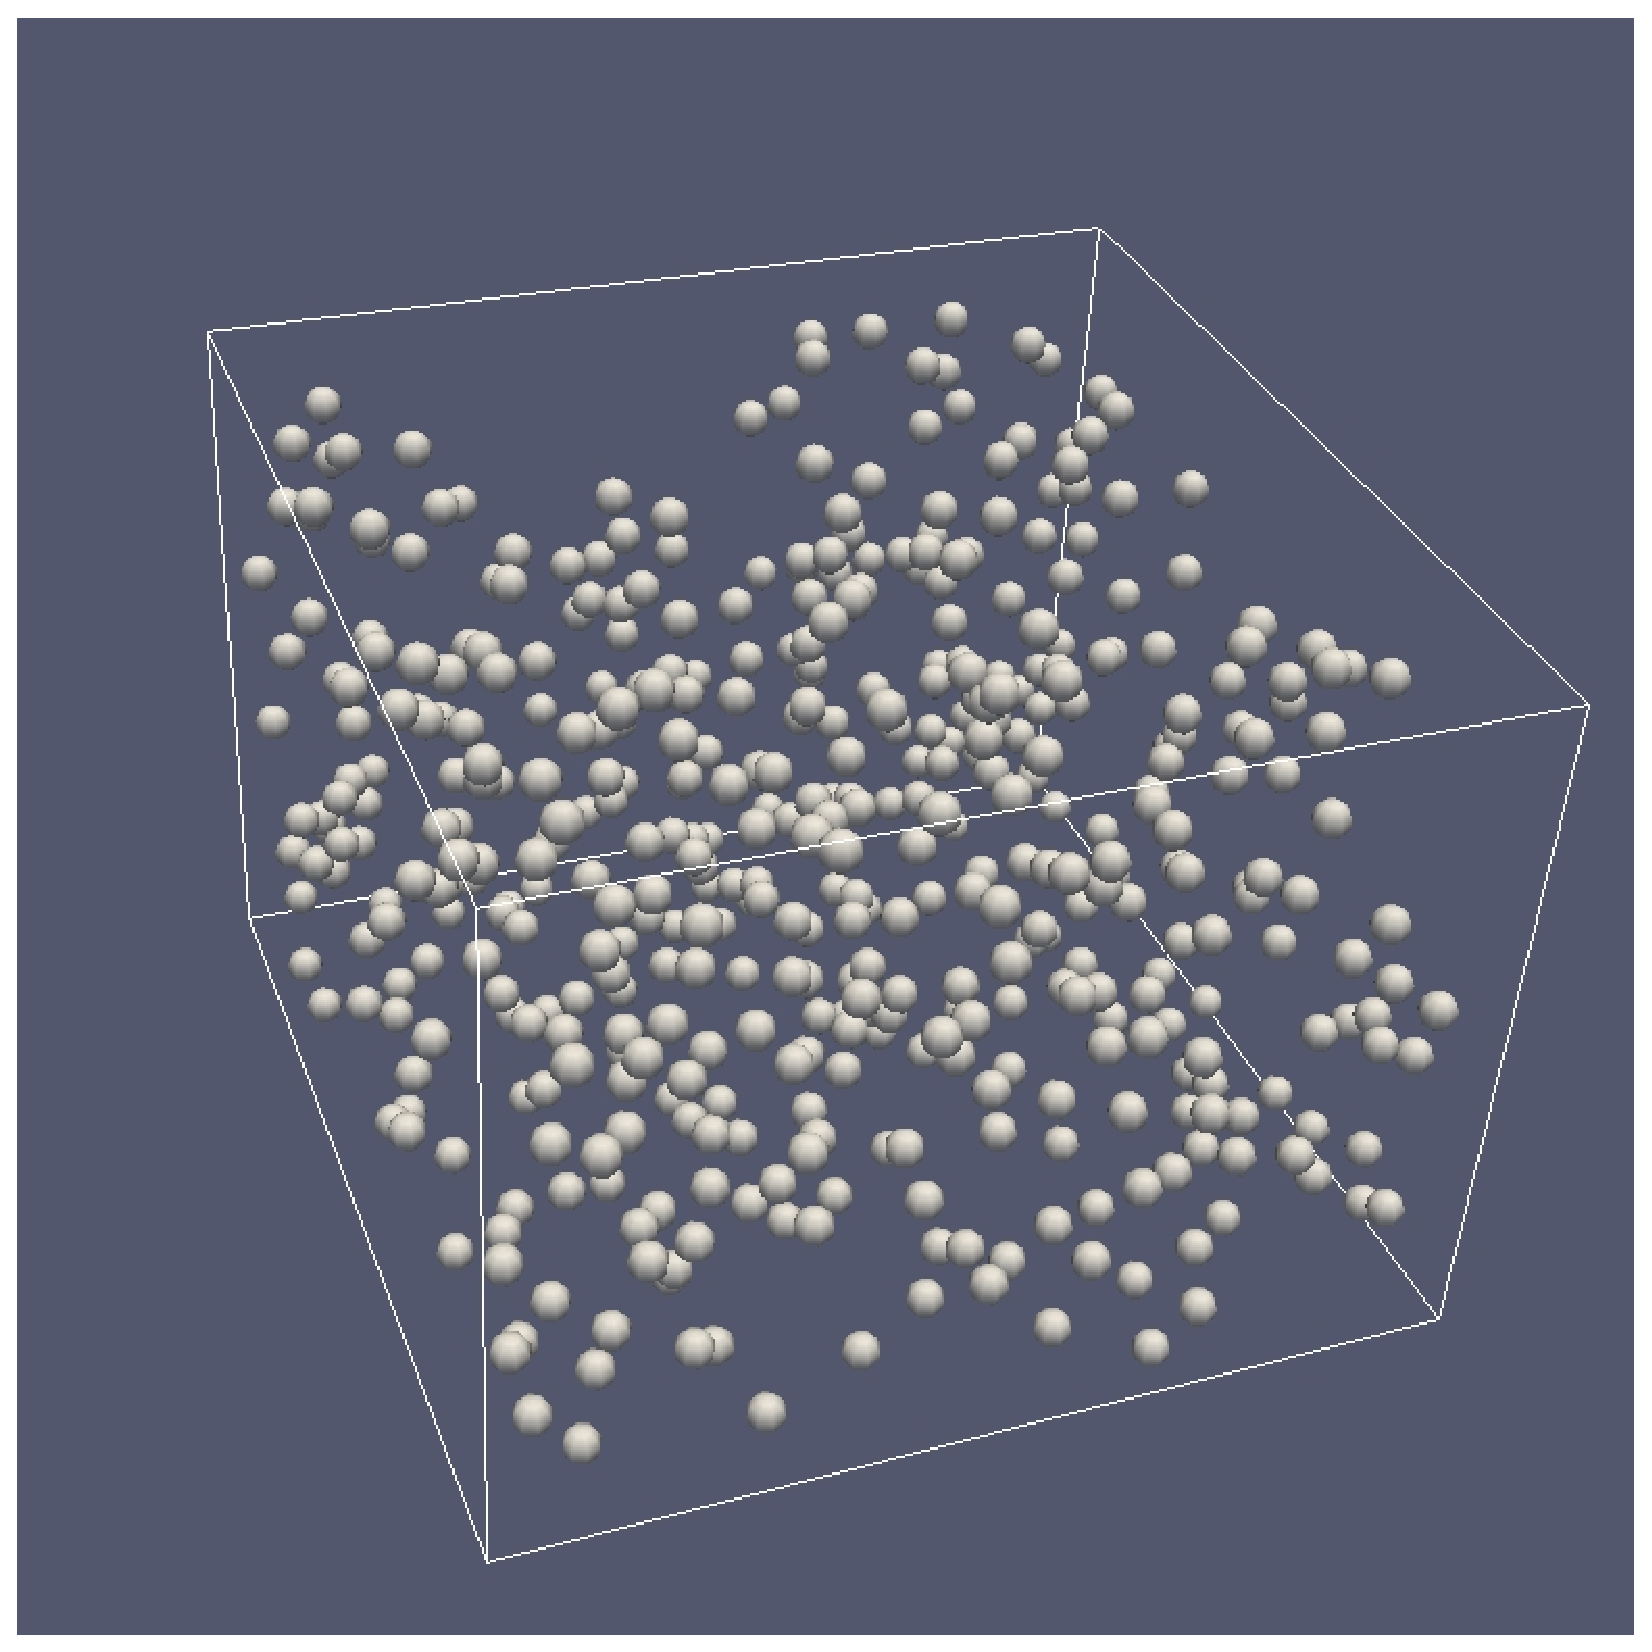
\includegraphics[width=\columnwidth]{compare_image_tracked3D_1}}%
	\only<3>{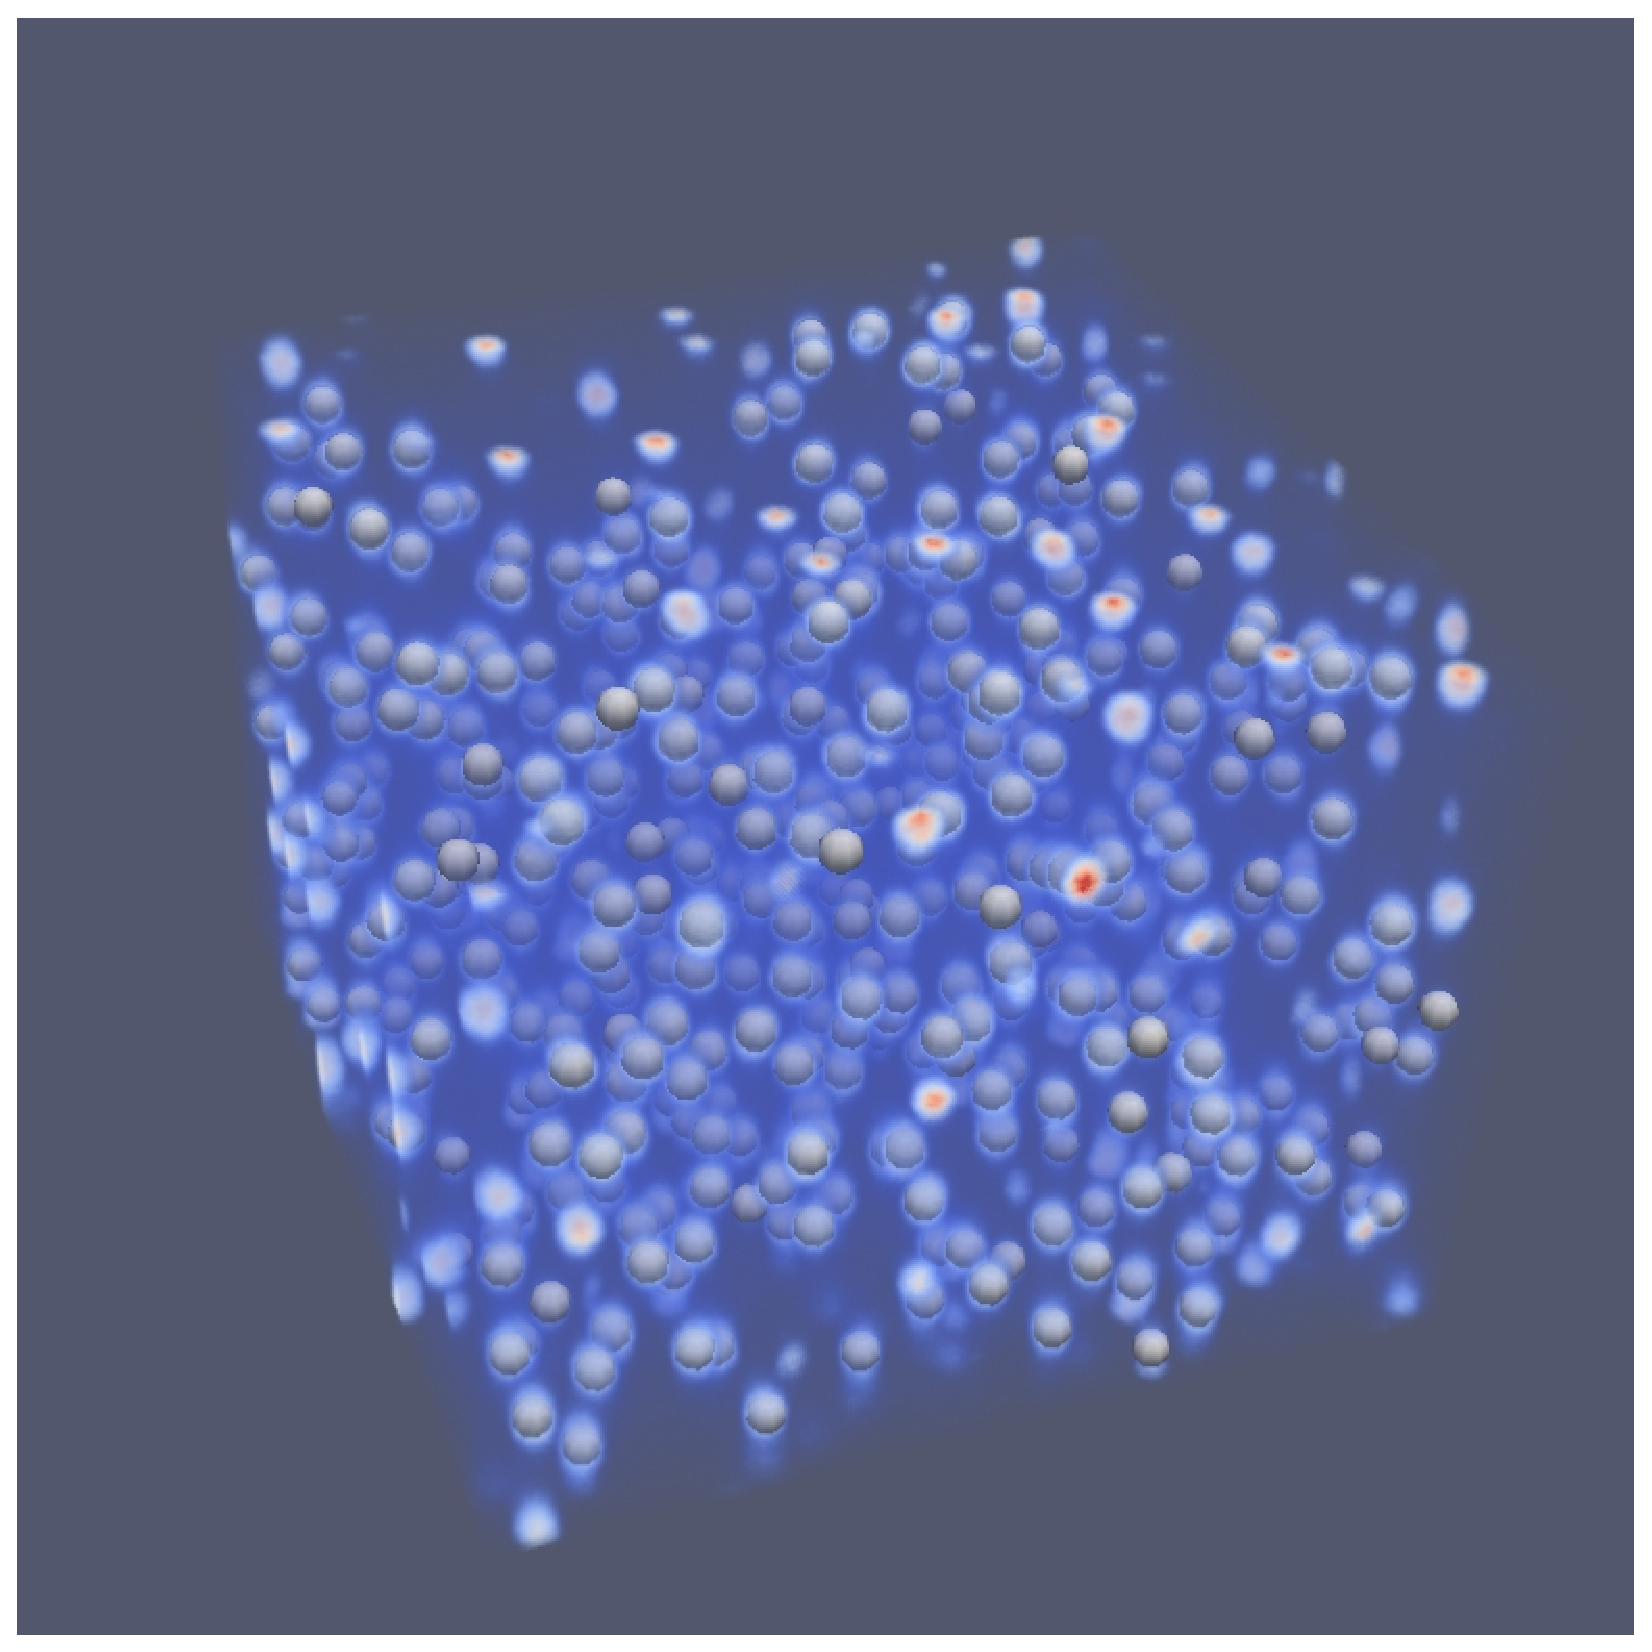
\includegraphics[width=\columnwidth]{compare_image_tracked3D_2}}\\
	\centering{\uncover<1,3>{Image}\uncover<3>{ $+$ }\uncover<2,3>{Tracked}}
	\column{0.3\textwidth}
	\begin{itemize}
		\item All particles are tracked
		\item Only particles are tracked
		\item Precision is about
	\end{itemize}
	\begin{align*}
		&\unit{0.1}{pixels}\\
		&\unit{0.01}{\sigma}\\
		&\unit{30}{\nano\metre}
	\end{align*}
	\end{columns}
\end{frame}

\subsection{Simulations}

\begin{frame}{Comparing with Brownian dynamics simulations}
	\begin{columns}
	\column{0.4\textwidth}
		\resizebox{\columnwidth}{!}{\begin{Large}% GNUPLOT: LaTeX picture with Postscript
\begingroup
  \makeatletter
  \providecommand\color[2][]{%
    \GenericError{(gnuplot) \space\space\space\@spaces}{%
      Package color not loaded in conjunction with
      terminal option `colourtext'%
    }{See the gnuplot documentation for explanation.%
    }{Either use 'blacktext' in gnuplot or load the package
      color.sty in LaTeX.}%
    \renewcommand\color[2][]{}%
  }%
  \providecommand\includegraphics[2][]{%
    \GenericError{(gnuplot) \space\space\space\@spaces}{%
      Package graphicx or graphics not loaded%
    }{See the gnuplot documentation for explanation.%
    }{The gnuplot epslatex terminal needs graphicx.sty or graphics.sty.}%
    \renewcommand\includegraphics[2][]{}%
  }%
  \providecommand\rotatebox[2]{#2}%
  \@ifundefined{ifGPcolor}{%
    \newif\ifGPcolor
    \GPcolortrue
  }{}%
  \@ifundefined{ifGPblacktext}{%
    \newif\ifGPblacktext
    \GPblacktexttrue
  }{}%
  % define a \g@addto@macro without @ in the name:
  \let\gplgaddtomacro\g@addto@macro
  % define empty templates for all commands taking text:
  \gdef\gplbacktext{}%
  \gdef\gplfronttext{}%
  \makeatother
  \ifGPblacktext
    % no textcolor at all
    \def\colorrgb#1{}%
    \def\colorgray#1{}%
  \else
    % gray or color?
    \ifGPcolor
      \def\colorrgb#1{\color[rgb]{#1}}%
      \def\colorgray#1{\color[gray]{#1}}%
      \expandafter\def\csname LTw\endcsname{\color{white}}%
      \expandafter\def\csname LTb\endcsname{\color{black}}%
      \expandafter\def\csname LTa\endcsname{\color{black}}%
      \expandafter\def\csname LT0\endcsname{\color[rgb]{1,0,0}}%
      \expandafter\def\csname LT1\endcsname{\color[rgb]{0,1,0}}%
      \expandafter\def\csname LT2\endcsname{\color[rgb]{0,0,1}}%
      \expandafter\def\csname LT3\endcsname{\color[rgb]{1,0,1}}%
      \expandafter\def\csname LT4\endcsname{\color[rgb]{0,1,1}}%
      \expandafter\def\csname LT5\endcsname{\color[rgb]{1,1,0}}%
      \expandafter\def\csname LT6\endcsname{\color[rgb]{0,0,0}}%
      \expandafter\def\csname LT7\endcsname{\color[rgb]{1,0.3,0}}%
      \expandafter\def\csname LT8\endcsname{\color[rgb]{0.5,0.5,0.5}}%
    \else
      % gray
      \def\colorrgb#1{\color{black}}%
      \def\colorgray#1{\color[gray]{#1}}%
      \expandafter\def\csname LTw\endcsname{\color{white}}%
      \expandafter\def\csname LTb\endcsname{\color{black}}%
      \expandafter\def\csname LTa\endcsname{\color{black}}%
      \expandafter\def\csname LT0\endcsname{\color{black}}%
      \expandafter\def\csname LT1\endcsname{\color{black}}%
      \expandafter\def\csname LT2\endcsname{\color{black}}%
      \expandafter\def\csname LT3\endcsname{\color{black}}%
      \expandafter\def\csname LT4\endcsname{\color{black}}%
      \expandafter\def\csname LT5\endcsname{\color{black}}%
      \expandafter\def\csname LT6\endcsname{\color{black}}%
      \expandafter\def\csname LT7\endcsname{\color{black}}%
      \expandafter\def\csname LT8\endcsname{\color{black}}%
    \fi
  \fi
  \setlength{\unitlength}{0.0500bp}%
  \begin{picture}(3600.00,5040.00)%
    \gplgaddtomacro\gplbacktext{%
      \csname LTb\endcsname%
      \put(660,704){\makebox(0,0)[r]{\strut{}$0$}}%
      \put(660,2740){\makebox(0,0)[r]{\strut{}$0.025$}}%
      \put(660,4776){\makebox(0,0)[r]{\strut{}$0.05$}}%
      \put(1266,484){\makebox(0,0){\strut{}$1$}}%
      \put(2213,484){\makebox(0,0){\strut{}$1.1$}}%
      \put(3160,484){\makebox(0,0){\strut{}$1.2$}}%
      \put(418,3840){\rotatebox{-270}{\makebox(0,0){\strut{}$U(r)/\epsilon$}}}%
      \put(3379,2740){\rotatebox{-270}{\makebox(0,0){\strut{}}}}%
      \put(1976,154){\makebox(0,0){\strut{}$r/\sigma$}}%
      \put(1976,4666){\makebox(0,0){\strut{}}}%
      \put(1976,4665){\makebox(0,0){\strut{}}}%
      \put(-396,110){\makebox(0,0)[l]{\strut{}}}%
      \put(1502,3147){\makebox(0,0){\strut{}$\frac{k_B T}{\epsilon}$}}%
      \put(2118,1722){\makebox(0,0)[r]{\strut{}$\sigma_{eff}$}}%
    }%
    \gplgaddtomacro\gplfronttext{%
    }%
    \gplbacktext
    \put(0,0){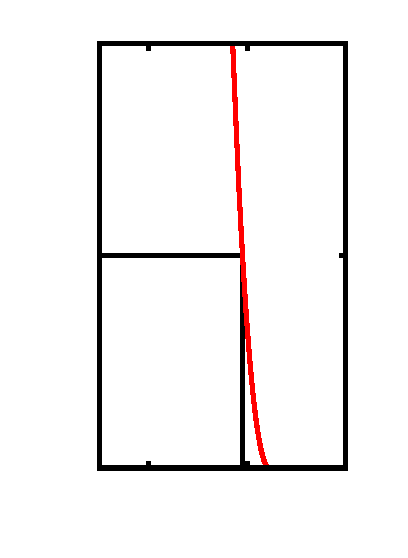
\includegraphics{wca}}%
    \gplfronttext
  \end{picture}%
\endgroup
\end{Large}}
	\column{0.6\textwidth}
	\begin{itemize}
		\item WCA potential: quasi hard-spheres
	\end{itemize}
	\[ U_{jk}(r) = \left\{\begin{array}{l l}
  		4\epsilon & \left[ \left( \frac{\sigma_{jk}}{r}\right)^{12} - \left( \frac{\sigma_{jk}}{r}\right)^{6} +\frac{1}{4}\right]  \\
  		& \quad \text{for }r<2^\frac{1}{6} \sigma_{jk}\\
  		0 & \quad \text{otherwise}
  	\end{array} \right. \]
  	\begin{itemize}
		\item Brownian $\simeq$ colloidal
		\item Gaussian polydispersity $\Delta=6\%$
		\item Periodic boundary conditions
	\end{itemize}
	
	\bigskip
	\footnotesize{Re-analysing simulations of Takeshi Kawasaki}
	\end{columns}
\end{frame}

\subsection{Dynamic signature}

\begin{frame}{Dynamic signature}
	\begin{columns}[T]
	\column{0.5\textwidth}
	\alt<1|handout:0>{\resizebox{\columnwidth}{0.7\columnwidth}{\input{isf_kob.pdf_tex}}}%
		{\resizebox{\textwidth}{!}{\begin{Large}% GNUPLOT: LaTeX picture with Postscript
\begingroup
  \makeatletter
  \providecommand\color[2][]{%
    \GenericError{(gnuplot) \space\space\space\@spaces}{%
      Package color not loaded in conjunction with
      terminal option `colourtext'%
    }{See the gnuplot documentation for explanation.%
    }{Either use 'blacktext' in gnuplot or load the package
      color.sty in LaTeX.}%
    \renewcommand\color[2][]{}%
  }%
  \providecommand\includegraphics[2][]{%
    \GenericError{(gnuplot) \space\space\space\@spaces}{%
      Package graphicx or graphics not loaded%
    }{See the gnuplot documentation for explanation.%
    }{The gnuplot epslatex terminal needs graphicx.sty or graphics.sty.}%
    \renewcommand\includegraphics[2][]{}%
  }%
  \providecommand\rotatebox[2]{#2}%
  \@ifundefined{ifGPcolor}{%
    \newif\ifGPcolor
    \GPcolortrue
  }{}%
  \@ifundefined{ifGPblacktext}{%
    \newif\ifGPblacktext
    \GPblacktexttrue
  }{}%
  % define a \g@addto@macro without @ in the name:
  \let\gplgaddtomacro\g@addto@macro
  % define empty templates for all commands taking text:
  \gdef\gplbacktext{}%
  \gdef\gplfronttext{}%
  \makeatother
  \ifGPblacktext
    % no textcolor at all
    \def\colorrgb#1{}%
    \def\colorgray#1{}%
  \else
    % gray or color?
    \ifGPcolor
      \def\colorrgb#1{\color[rgb]{#1}}%
      \def\colorgray#1{\color[gray]{#1}}%
      \expandafter\def\csname LTw\endcsname{\color{white}}%
      \expandafter\def\csname LTb\endcsname{\color{black}}%
      \expandafter\def\csname LTa\endcsname{\color{black}}%
      \expandafter\def\csname LT0\endcsname{\color[rgb]{1,0,0}}%
      \expandafter\def\csname LT1\endcsname{\color[rgb]{0,1,0}}%
      \expandafter\def\csname LT2\endcsname{\color[rgb]{0,0,1}}%
      \expandafter\def\csname LT3\endcsname{\color[rgb]{1,0,1}}%
      \expandafter\def\csname LT4\endcsname{\color[rgb]{0,1,1}}%
      \expandafter\def\csname LT5\endcsname{\color[rgb]{1,1,0}}%
      \expandafter\def\csname LT6\endcsname{\color[rgb]{0,0,0}}%
      \expandafter\def\csname LT7\endcsname{\color[rgb]{1,0.3,0}}%
      \expandafter\def\csname LT8\endcsname{\color[rgb]{0.5,0.5,0.5}}%
    \else
      % gray
      \def\colorrgb#1{\color{black}}%
      \def\colorgray#1{\color[gray]{#1}}%
      \expandafter\def\csname LTw\endcsname{\color{white}}%
      \expandafter\def\csname LTb\endcsname{\color{black}}%
      \expandafter\def\csname LTa\endcsname{\color{black}}%
      \expandafter\def\csname LT0\endcsname{\color{black}}%
      \expandafter\def\csname LT1\endcsname{\color{black}}%
      \expandafter\def\csname LT2\endcsname{\color{black}}%
      \expandafter\def\csname LT3\endcsname{\color{black}}%
      \expandafter\def\csname LT4\endcsname{\color{black}}%
      \expandafter\def\csname LT5\endcsname{\color{black}}%
      \expandafter\def\csname LT6\endcsname{\color{black}}%
      \expandafter\def\csname LT7\endcsname{\color{black}}%
      \expandafter\def\csname LT8\endcsname{\color{black}}%
    \fi
  \fi
  \setlength{\unitlength}{0.0500bp}%
  \begin{picture}(7200.00,5040.00)%
    \gplgaddtomacro\gplbacktext{%
      \csname LTb\endcsname%
      \put(1056,1518){\makebox(0,0)[r]{\strut{}$0.2$}}%
      \put(1056,2333){\makebox(0,0)[r]{\strut{}$0.4$}}%
      \put(1056,3147){\makebox(0,0)[r]{\strut{}$0.6$}}%
      \put(1056,3962){\makebox(0,0)[r]{\strut{}$0.8$}}%
      \put(1056,4776){\makebox(0,0)[r]{\strut{}$1$}}%
      \put(1251,484){\makebox(0,0){\strut{}$10^{0}$}}%
      \put(2628,484){\makebox(0,0){\strut{}$10^{1}$}}%
      \put(4006,484){\makebox(0,0){\strut{}$10^{2}$}}%
      \put(5383,484){\makebox(0,0){\strut{}$10^{3}$}}%
      \put(6760,484){\makebox(0,0){\strut{}$10^{4}$}}%
      \put(418,2740){\rotatebox{-270}{\makebox(0,0){\strut{}Self \ac{ISF}}}}%
      \put(6979,2740){\rotatebox{-270}{\makebox(0,0){\strut{}}}}%
      \put(3974,154){\makebox(0,0){\strut{}$t/\tau_B$}}%
      \put(3974,4666){\makebox(0,0){\strut{}}}%
      \put(3974,4665){\makebox(0,0){\strut{}}}%
      \put(264,110){\makebox(0,0)[l]{\strut{}}}%
    }%
    \gplgaddtomacro\gplfronttext{%
      \csname LTb\endcsname%
      \put(6037,3525){\makebox(0,0)[r]{\strut{}$\phi=0.497$}}%
      \csname LTb\endcsname%
      \put(6037,3789){\makebox(0,0)[r]{\strut{}$\phi=0.535$}}%
      \csname LTb\endcsname%
      \put(6037,4053){\makebox(0,0)[r]{\strut{}$\phi=0.540$}}%
      \csname LTb\endcsname%
      \put(6037,4317){\makebox(0,0)[r]{\strut{}$\phi=0.555$}}%
      \csname LTb\endcsname%
      \put(6037,4581){\makebox(0,0)[r]{\strut{}$\phi=0.576$}}%
    }%
    \gplbacktext
    \put(0,0){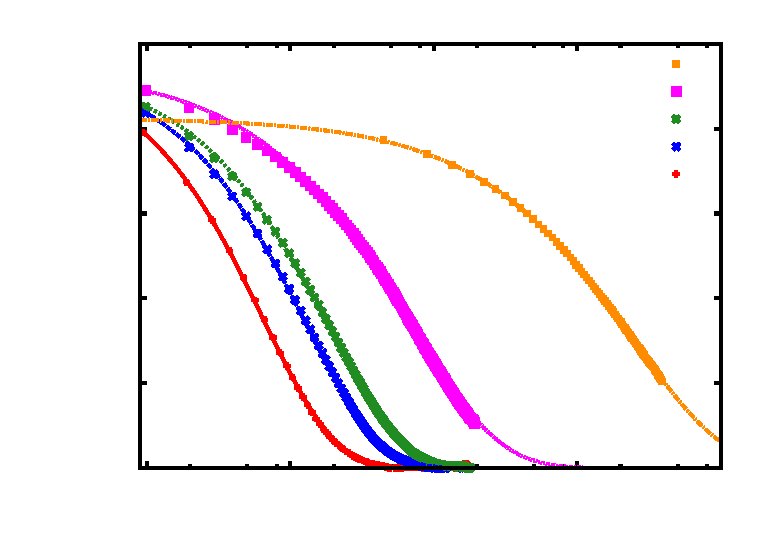
\includegraphics{./fit_isf}}%
    \gplfronttext
  \end{picture}%
\endgroup
\end{Large}}}%
	\begin{itemize}
		\item Dramatic slowing down
		\item Two step relaxation
		\item Plateau
		\item VFT fit $\Rightarrow\phi_0$
		\item<4> Good agreement with simulations
	\end{itemize}
	\column{0.5\textwidth}
	\alt<3->{\resizebox{\textwidth}{!}{\begin{Large}% GNUPLOT: LaTeX picture with Postscript
\begingroup
  \makeatletter
  \providecommand\color[2][]{%
    \GenericError{(gnuplot) \space\space\space\@spaces}{%
      Package color not loaded in conjunction with
      terminal option `colourtext'%
    }{See the gnuplot documentation for explanation.%
    }{Either use 'blacktext' in gnuplot or load the package
      color.sty in LaTeX.}%
    \renewcommand\color[2][]{}%
  }%
  \providecommand\includegraphics[2][]{%
    \GenericError{(gnuplot) \space\space\space\@spaces}{%
      Package graphicx or graphics not loaded%
    }{See the gnuplot documentation for explanation.%
    }{The gnuplot epslatex terminal needs graphicx.sty or graphics.sty.}%
    \renewcommand\includegraphics[2][]{}%
  }%
  \providecommand\rotatebox[2]{#2}%
  \@ifundefined{ifGPcolor}{%
    \newif\ifGPcolor
    \GPcolortrue
  }{}%
  \@ifundefined{ifGPblacktext}{%
    \newif\ifGPblacktext
    \GPblacktexttrue
  }{}%
  % define a \g@addto@macro without @ in the name:
  \let\gplgaddtomacro\g@addto@macro
  % define empty templates for all commands taking text:
  \gdef\gplbacktext{}%
  \gdef\gplfronttext{}%
  \makeatother
  \ifGPblacktext
    % no textcolor at all
    \def\colorrgb#1{}%
    \def\colorgray#1{}%
  \else
    % gray or color?
    \ifGPcolor
      \def\colorrgb#1{\color[rgb]{#1}}%
      \def\colorgray#1{\color[gray]{#1}}%
      \expandafter\def\csname LTw\endcsname{\color{white}}%
      \expandafter\def\csname LTb\endcsname{\color{black}}%
      \expandafter\def\csname LTa\endcsname{\color{black}}%
      \expandafter\def\csname LT0\endcsname{\color[rgb]{1,0,0}}%
      \expandafter\def\csname LT1\endcsname{\color[rgb]{0,1,0}}%
      \expandafter\def\csname LT2\endcsname{\color[rgb]{0,0,1}}%
      \expandafter\def\csname LT3\endcsname{\color[rgb]{1,0,1}}%
      \expandafter\def\csname LT4\endcsname{\color[rgb]{0,1,1}}%
      \expandafter\def\csname LT5\endcsname{\color[rgb]{1,1,0}}%
      \expandafter\def\csname LT6\endcsname{\color[rgb]{0,0,0}}%
      \expandafter\def\csname LT7\endcsname{\color[rgb]{1,0.3,0}}%
      \expandafter\def\csname LT8\endcsname{\color[rgb]{0.5,0.5,0.5}}%
    \else
      % gray
      \def\colorrgb#1{\color{black}}%
      \def\colorgray#1{\color[gray]{#1}}%
      \expandafter\def\csname LTw\endcsname{\color{white}}%
      \expandafter\def\csname LTb\endcsname{\color{black}}%
      \expandafter\def\csname LTa\endcsname{\color{black}}%
      \expandafter\def\csname LT0\endcsname{\color{black}}%
      \expandafter\def\csname LT1\endcsname{\color{black}}%
      \expandafter\def\csname LT2\endcsname{\color{black}}%
      \expandafter\def\csname LT3\endcsname{\color{black}}%
      \expandafter\def\csname LT4\endcsname{\color{black}}%
      \expandafter\def\csname LT5\endcsname{\color{black}}%
      \expandafter\def\csname LT6\endcsname{\color{black}}%
      \expandafter\def\csname LT7\endcsname{\color{black}}%
      \expandafter\def\csname LT8\endcsname{\color{black}}%
    \fi
  \fi
  \setlength{\unitlength}{0.0500bp}%
  \begin{picture}(7200.00,5040.00)%
    \gplgaddtomacro\gplbacktext{%
      \csname LTb\endcsname%
      \put(1056,704){\makebox(0,0)[r]{\strut{}$10^{-2}$}}%
      \put(1056,2061){\makebox(0,0)[r]{\strut{}$10^{-1}$}}%
      \put(1056,3419){\makebox(0,0)[r]{\strut{}$10^{0}$}}%
      \put(1056,4776){\makebox(0,0)[r]{\strut{}$10^{1}$}}%
      \put(1251,484){\makebox(0,0){\strut{}$10^{0}$}}%
      \put(2628,484){\makebox(0,0){\strut{}$10^{1}$}}%
      \put(4006,484){\makebox(0,0){\strut{}$10^{2}$}}%
      \put(5383,484){\makebox(0,0){\strut{}$10^{3}$}}%
      \put(6760,484){\makebox(0,0){\strut{}$10^{4}$}}%
      \put(286,2740){\rotatebox{-270}{\makebox(0,0){\strut{}$\Delta r^2/\sigma^2$}}}%
      \put(6979,2740){\rotatebox{-270}{\makebox(0,0){\strut{}}}}%
      \put(3974,154){\makebox(0,0){\strut{}$t/\tau_B$}}%
      \put(3974,4666){\makebox(0,0){\strut{}}}%
      \put(3974,4665){\makebox(0,0){\strut{}}}%
      \put(-264,110){\makebox(0,0)[l]{\strut{}}}%
    }%
    \gplgaddtomacro\gplfronttext{%
      \csname LTb\endcsname%
      \put(2904,4581){\makebox(0,0)[r]{\strut{}$\phi=0.497$}}%
      \csname LTb\endcsname%
      \put(2904,4317){\makebox(0,0)[r]{\strut{}$\phi=0.535$}}%
      \csname LTb\endcsname%
      \put(2904,4053){\makebox(0,0)[r]{\strut{}$\phi=0.540$}}%
      \csname LTb\endcsname%
      \put(2904,3789){\makebox(0,0)[r]{\strut{}$\phi=0.555$}}%
      \csname LTb\endcsname%
      \put(2904,3525){\makebox(0,0)[r]{\strut{}$\phi=0.576$}}%
    }%
    \gplbacktext
    \put(0,0){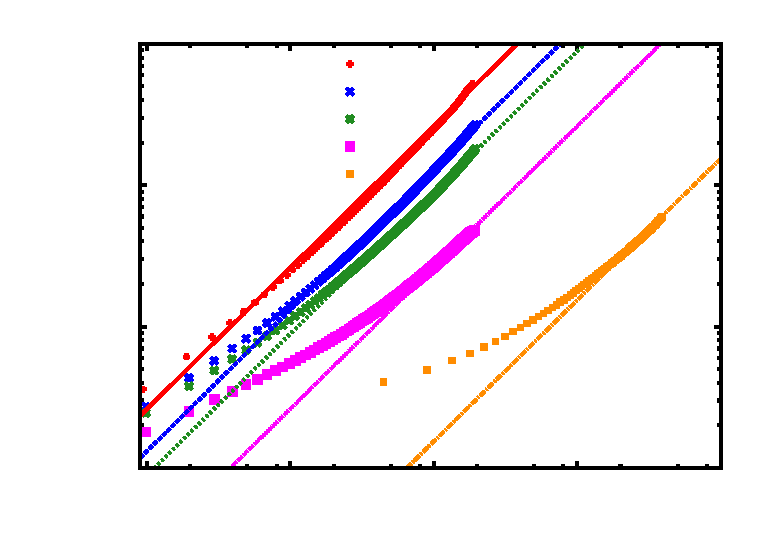
\includegraphics{./fit_msd}}%
    \gplfronttext
  \end{picture}%
\endgroup
\end{Large}}}%
	{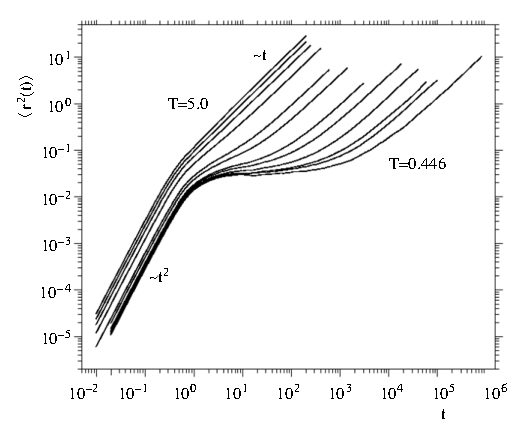
\includegraphics[width=\columnwidth, height=0.7\columnwidth]{msd_kob}}\\
	\alt<4>{\resizebox{\textwidth}{!}{\begin{Large}% GNUPLOT: LaTeX picture with Postscript
\begingroup
  \makeatletter
  \providecommand\color[2][]{%
    \GenericError{(gnuplot) \space\space\space\@spaces}{%
      Package color not loaded in conjunction with
      terminal option `colourtext'%
    }{See the gnuplot documentation for explanation.%
    }{Either use 'blacktext' in gnuplot or load the package
      color.sty in LaTeX.}%
    \renewcommand\color[2][]{}%
  }%
  \providecommand\includegraphics[2][]{%
    \GenericError{(gnuplot) \space\space\space\@spaces}{%
      Package graphicx or graphics not loaded%
    }{See the gnuplot documentation for explanation.%
    }{The gnuplot epslatex terminal needs graphicx.sty or graphics.sty.}%
    \renewcommand\includegraphics[2][]{}%
  }%
  \providecommand\rotatebox[2]{#2}%
  \@ifundefined{ifGPcolor}{%
    \newif\ifGPcolor
    \GPcolortrue
  }{}%
  \@ifundefined{ifGPblacktext}{%
    \newif\ifGPblacktext
    \GPblacktexttrue
  }{}%
  % define a \g@addto@macro without @ in the name:
  \let\gplgaddtomacro\g@addto@macro
  % define empty templates for all commands taking text:
  \gdef\gplbacktext{}%
  \gdef\gplfronttext{}%
  \makeatother
  \ifGPblacktext
    % no textcolor at all
    \def\colorrgb#1{}%
    \def\colorgray#1{}%
  \else
    % gray or color?
    \ifGPcolor
      \def\colorrgb#1{\color[rgb]{#1}}%
      \def\colorgray#1{\color[gray]{#1}}%
      \expandafter\def\csname LTw\endcsname{\color{white}}%
      \expandafter\def\csname LTb\endcsname{\color{black}}%
      \expandafter\def\csname LTa\endcsname{\color{black}}%
      \expandafter\def\csname LT0\endcsname{\color[rgb]{1,0,0}}%
      \expandafter\def\csname LT1\endcsname{\color[rgb]{0,1,0}}%
      \expandafter\def\csname LT2\endcsname{\color[rgb]{0,0,1}}%
      \expandafter\def\csname LT3\endcsname{\color[rgb]{1,0,1}}%
      \expandafter\def\csname LT4\endcsname{\color[rgb]{0,1,1}}%
      \expandafter\def\csname LT5\endcsname{\color[rgb]{1,1,0}}%
      \expandafter\def\csname LT6\endcsname{\color[rgb]{0,0,0}}%
      \expandafter\def\csname LT7\endcsname{\color[rgb]{1,0.3,0}}%
      \expandafter\def\csname LT8\endcsname{\color[rgb]{0.5,0.5,0.5}}%
    \else
      % gray
      \def\colorrgb#1{\color{black}}%
      \def\colorgray#1{\color[gray]{#1}}%
      \expandafter\def\csname LTw\endcsname{\color{white}}%
      \expandafter\def\csname LTb\endcsname{\color{black}}%
      \expandafter\def\csname LTa\endcsname{\color{black}}%
      \expandafter\def\csname LT0\endcsname{\color{black}}%
      \expandafter\def\csname LT1\endcsname{\color{black}}%
      \expandafter\def\csname LT2\endcsname{\color{black}}%
      \expandafter\def\csname LT3\endcsname{\color{black}}%
      \expandafter\def\csname LT4\endcsname{\color{black}}%
      \expandafter\def\csname LT5\endcsname{\color{black}}%
      \expandafter\def\csname LT6\endcsname{\color{black}}%
      \expandafter\def\csname LT7\endcsname{\color{black}}%
      \expandafter\def\csname LT8\endcsname{\color{black}}%
    \fi
  \fi
  \setlength{\unitlength}{0.0500bp}%
  \begin{picture}(7200.00,5040.00)%
    \gplgaddtomacro\gplbacktext{%
      \csname LTb\endcsname%
      \put(1056,704){\makebox(0,0)[r]{\strut{}$10^{0}$}}%
      \put(1056,1722){\makebox(0,0)[r]{\strut{}$10^{1}$}}%
      \put(1056,2740){\makebox(0,0)[r]{\strut{}$10^{2}$}}%
      \put(1056,3758){\makebox(0,0)[r]{\strut{}$10^{3}$}}%
      \put(1056,4776){\makebox(0,0)[r]{\strut{}$10^{4}$}}%
      \put(1967,484){\makebox(0,0){\strut{}$0.50$}}%
      \put(3165,484){\makebox(0,0){\strut{}$0.52$}}%
      \put(4363,484){\makebox(0,0){\strut{}$0.54$}}%
      \put(5562,484){\makebox(0,0){\strut{}$0.56$}}%
      \put(6760,484){\makebox(0,0){\strut{}$0.58$}}%
      \put(418,2740){\rotatebox{-270}{\makebox(0,0){\strut{}$t/\tau_B$}}}%
      \put(6979,2740){\rotatebox{-270}{\makebox(0,0){\strut{}}}}%
      \put(3974,154){\makebox(0,0){\strut{}$\phi$}}%
      \put(3974,4666){\makebox(0,0){\strut{}}}%
      \put(3974,4665){\makebox(0,0){\strut{}}}%
      \put(-132,110){\makebox(0,0)[l]{\strut{}}}%
    }%
    \gplgaddtomacro\gplfronttext{%
      \csname LTb\endcsname%
      \put(4620,4556){\makebox(0,0)[r]{\strut{}$\tau_\alpha$ experiments}}%
      \csname LTb\endcsname%
      \put(4620,4241){\makebox(0,0)[r]{\strut{}$\tau_\alpha$ simulations}}%
    }%
    \gplbacktext
    \put(0,0){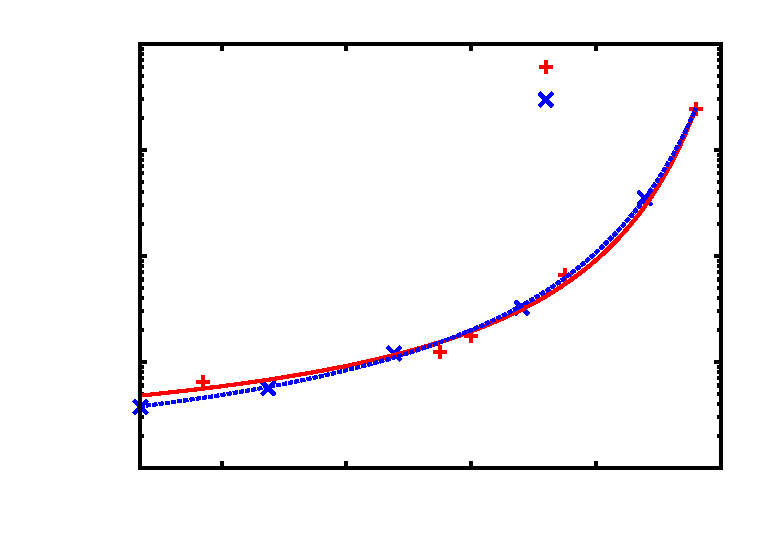
\includegraphics{fit_tau_alpha_vft}}%
    \gplfronttext
  \end{picture}%
\endgroup
\end{Large}}}%
		{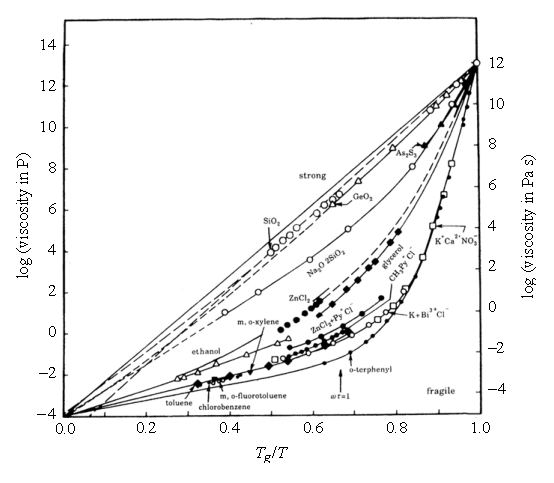
\includegraphics[width=\columnwidth, height=0.7\columnwidth]{angell}}
	\end{columns}
\end{frame}

\begin{frame}<all:1->{Dynamic heterogeneities}
	\begin{textblock*}{0.6\textwidth}(10mm,92mm)
		\simplephasediagram{%
		\node<all:1> at (0.497,0) [xp marker, fill=green!50!black] {};
		\node<all:2> at (0.535,0) [xp marker, fill=green!50!black] {};
		\node<all:3> at (0.576,0) [xp marker, fill=green!50!black] {};
		}
	\end{textblock*}
	\begin{columns}[T]
	\column{0.6\textwidth}
	\only<all:1>{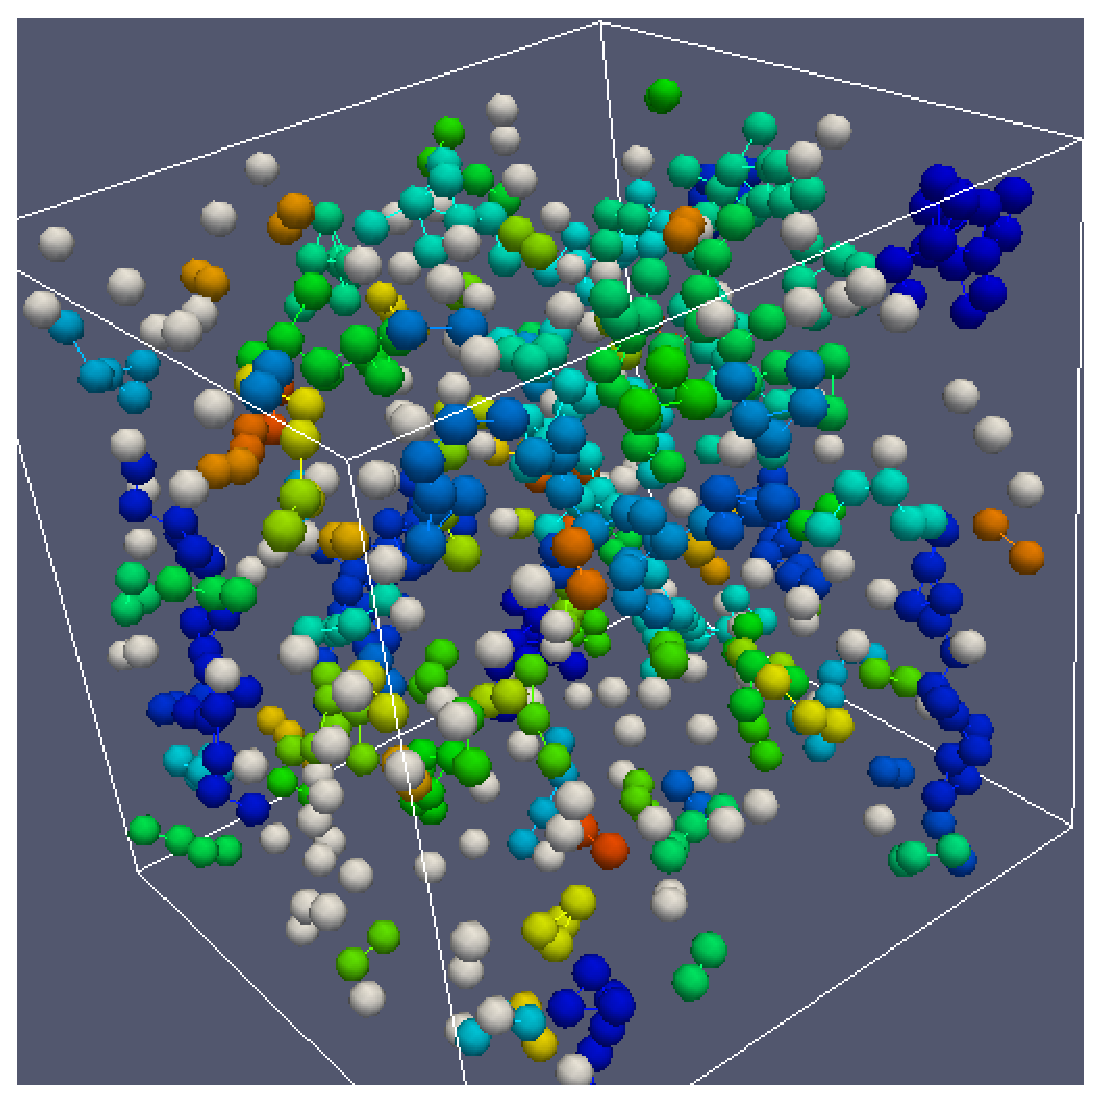
\includegraphics[width=\columnwidth]{dh_3954}
	\[ \phi=0.497 \]}%
	\only<all:2>{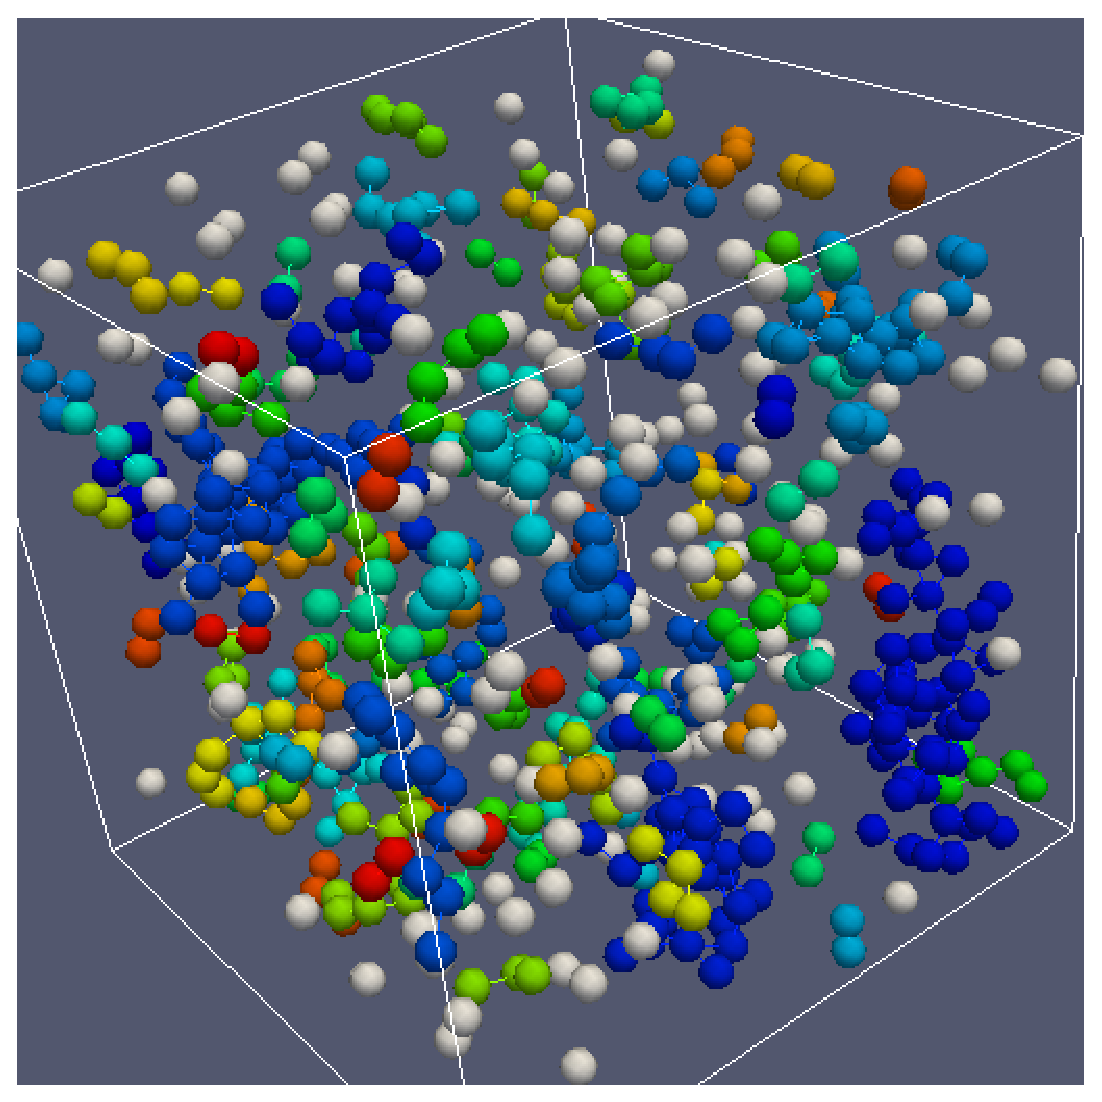
\includegraphics[width=\columnwidth]{dh_4582}
	\[ \phi=0.535 \]}%
	\only<all:3>{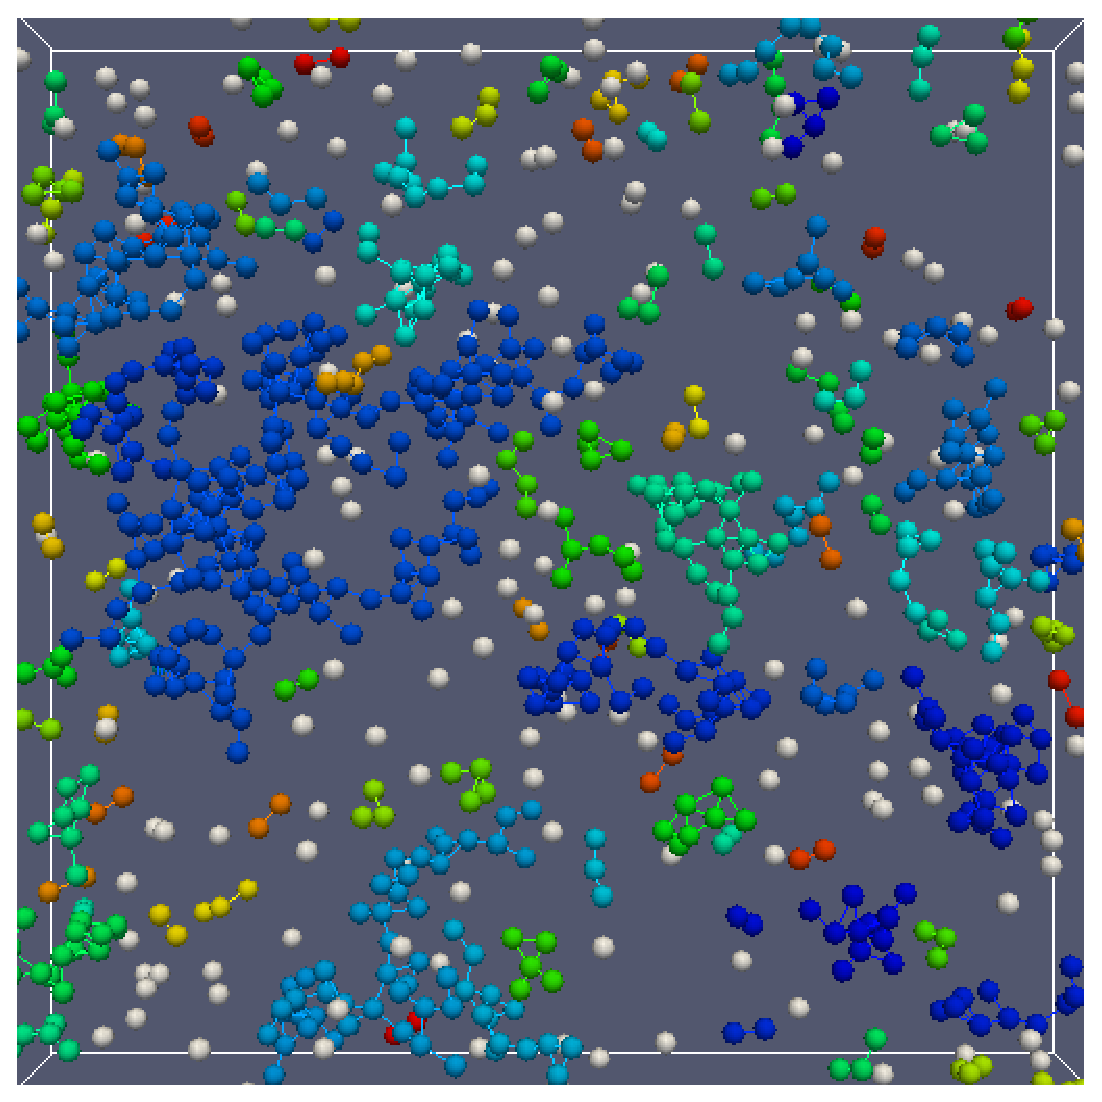
\includegraphics[width=\columnwidth]{dh_go1}
	\[ \phi=0.576 \]}%
	\column{0.4\textwidth}
	\begin{block}{$10\%$ fastest particles}
	\begin{itemize}
		\item isolated \tikz\shade[ball color=white] (0,0) circle (0.5em);
		\item connected 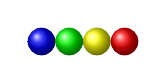
\begin{tikzpicture}
			\shade[ball color=blue] (0,0) circle (0.5em);
			\shade[ball color=green] +(1em,0) circle (0.5em);
			\shade[ball color=yellow] +(2em,0) circle (0.5em);
			\shade[ball color=red] +(3em,0) circle (0.5em);
			\end{tikzpicture}
	\end{itemize}
	\end{block}
	\begin{itemize}
		\item Rearrangements group in space
		\item Growing characteristic size
	\end{itemize}
	\end{columns}
\end{frame}

\begin{frame}{Dynamic correlation length}
	\begin{textblock*}{0.6\textwidth}(10mm,92mm)
		\simplephasediagram{}
	\end{textblock*}
	Spatial correlation of the fluctuations of the displacement
	\begin{columns}
	\column{0.6\textwidth}
	\[ \mathcal{G}_u(r,t) \equiv \frac{
		\left\langle \sum_{i,j}{\delta u_i(t) \delta u_j(t) \delta(r_{ij} -r)} \right\rangle 
	}{
		\left\langle \sum_{i,j}{\delta(r_{ij} -r)} \right\rangle
	}\]
	\column{0.4\textwidth}
	\begin{align*}
		u_i(t) \equiv & \|\vec{r}_i(t)-\vec{r}_i(0)\|\\
		\delta u_i \equiv& u_i- \langle u_i \rangle
	\end{align*}
	\end{columns}
	\begin{columns}
	\column{0.6\textwidth}
	\resizebox{\columnwidth}{!}{\begin{Large}% GNUPLOT: LaTeX picture with Postscript
\begingroup
  \makeatletter
  \providecommand\color[2][]{%
    \GenericError{(gnuplot) \space\space\space\@spaces}{%
      Package color not loaded in conjunction with
      terminal option `colourtext'%
    }{See the gnuplot documentation for explanation.%
    }{Either use 'blacktext' in gnuplot or load the package
      color.sty in LaTeX.}%
    \renewcommand\color[2][]{}%
  }%
  \providecommand\includegraphics[2][]{%
    \GenericError{(gnuplot) \space\space\space\@spaces}{%
      Package graphicx or graphics not loaded%
    }{See the gnuplot documentation for explanation.%
    }{The gnuplot epslatex terminal needs graphicx.sty or graphics.sty.}%
    \renewcommand\includegraphics[2][]{}%
  }%
  \providecommand\rotatebox[2]{#2}%
  \@ifundefined{ifGPcolor}{%
    \newif\ifGPcolor
    \GPcolortrue
  }{}%
  \@ifundefined{ifGPblacktext}{%
    \newif\ifGPblacktext
    \GPblacktexttrue
  }{}%
  % define a \g@addto@macro without @ in the name:
  \let\gplgaddtomacro\g@addto@macro
  % define empty templates for all commands taking text:
  \gdef\gplbacktext{}%
  \gdef\gplfronttext{}%
  \makeatother
  \ifGPblacktext
    % no textcolor at all
    \def\colorrgb#1{}%
    \def\colorgray#1{}%
  \else
    % gray or color?
    \ifGPcolor
      \def\colorrgb#1{\color[rgb]{#1}}%
      \def\colorgray#1{\color[gray]{#1}}%
      \expandafter\def\csname LTw\endcsname{\color{white}}%
      \expandafter\def\csname LTb\endcsname{\color{black}}%
      \expandafter\def\csname LTa\endcsname{\color{black}}%
      \expandafter\def\csname LT0\endcsname{\color[rgb]{1,0,0}}%
      \expandafter\def\csname LT1\endcsname{\color[rgb]{0,1,0}}%
      \expandafter\def\csname LT2\endcsname{\color[rgb]{0,0,1}}%
      \expandafter\def\csname LT3\endcsname{\color[rgb]{1,0,1}}%
      \expandafter\def\csname LT4\endcsname{\color[rgb]{0,1,1}}%
      \expandafter\def\csname LT5\endcsname{\color[rgb]{1,1,0}}%
      \expandafter\def\csname LT6\endcsname{\color[rgb]{0,0,0}}%
      \expandafter\def\csname LT7\endcsname{\color[rgb]{1,0.3,0}}%
      \expandafter\def\csname LT8\endcsname{\color[rgb]{0.5,0.5,0.5}}%
    \else
      % gray
      \def\colorrgb#1{\color{black}}%
      \def\colorgray#1{\color[gray]{#1}}%
      \expandafter\def\csname LTw\endcsname{\color{white}}%
      \expandafter\def\csname LTb\endcsname{\color{black}}%
      \expandafter\def\csname LTa\endcsname{\color{black}}%
      \expandafter\def\csname LT0\endcsname{\color{black}}%
      \expandafter\def\csname LT1\endcsname{\color{black}}%
      \expandafter\def\csname LT2\endcsname{\color{black}}%
      \expandafter\def\csname LT3\endcsname{\color{black}}%
      \expandafter\def\csname LT4\endcsname{\color{black}}%
      \expandafter\def\csname LT5\endcsname{\color{black}}%
      \expandafter\def\csname LT6\endcsname{\color{black}}%
      \expandafter\def\csname LT7\endcsname{\color{black}}%
      \expandafter\def\csname LT8\endcsname{\color{black}}%
    \fi
  \fi
  \setlength{\unitlength}{0.0500bp}%
  \begin{picture}(7200.00,5040.00)%
    \gplgaddtomacro\gplbacktext{%
      \csname LTb\endcsname%
      \put(1056,704){\makebox(0,0)[r]{\strut{}$10^{-4}$}}%
      \put(1056,1938){\makebox(0,0)[r]{\strut{}$10^{-3}$}}%
      \put(1056,3171){\makebox(0,0)[r]{\strut{}$10^{-2}$}}%
      \put(1056,4405){\makebox(0,0)[r]{\strut{}$10^{-1}$}}%
      \put(1368,484){\makebox(0,0){\strut{}$2$}}%
      \put(2266,484){\makebox(0,0){\strut{}$3$}}%
      \put(3165,484){\makebox(0,0){\strut{}$4$}}%
      \put(4064,484){\makebox(0,0){\strut{}$5$}}%
      \put(4963,484){\makebox(0,0){\strut{}$6$}}%
      \put(5861,484){\makebox(0,0){\strut{}$7$}}%
      \put(6760,484){\makebox(0,0){\strut{}$8$}}%
      \put(286,2740){\rotatebox{-270}{\makebox(0,0){\strut{}$\mathcal{G}_u(r,t^{dh})/\Delta r^2(t^{dh})$}}}%
      \put(6979,2740){\rotatebox{-270}{\makebox(0,0){\strut{}}}}%
      \put(3974,154){\makebox(0,0){\strut{}$r/\sigma$}}%
      \put(3974,4666){\makebox(0,0){\strut{}}}%
      \put(3974,4665){\makebox(0,0){\strut{}}}%
      \put(-264,110){\makebox(0,0)[l]{\strut{}}}%
    }%
    \gplgaddtomacro\gplfronttext{%
      \csname LTb\endcsname%
      \put(2904,932){\makebox(0,0)[r]{\strut{}$\phi=0.497$}}%
      \csname LTb\endcsname%
      \put(2904,1262){\makebox(0,0)[r]{\strut{}$\phi=0.555$}}%
      \csname LTb\endcsname%
      \put(2904,1592){\makebox(0,0)[r]{\strut{}$\phi=0.576$}}%
    }%
    \gplbacktext
    \put(0,0){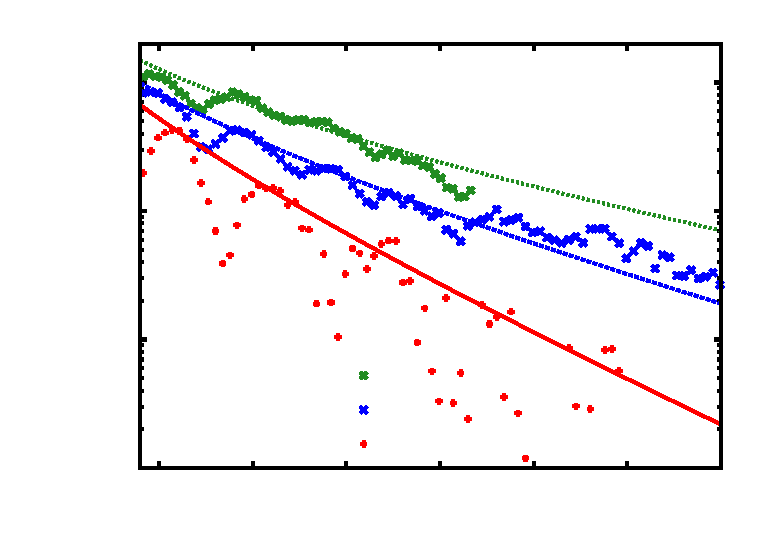
\includegraphics{fit_gu}}%
    \gplfronttext
  \end{picture}%
\endgroup
\end{Large}}
	\column{0.4\textwidth}
	Ornstein-Zernike fit
	\[ \mathcal{G}_u(r,t^{dh}) \propto r^{-1}\exp( -\frac{r}{\xi_u} )\]
	$\xi_u$ grows when approaching the glass transition
	\end{columns}
\end{frame}

\begin{frame}{Our system}
	\begin{itemize}
		\item Exhibits the phenomenology of the glass transition
		\item Is a valid model system
		\item Allows access to the scale of its elementary particles
	\end{itemize}
	\bigskip $\Rightarrow$ We can investigate both the dynamics and the structure at the particle level
\end{frame}